%%=============================================================================
%% Opstelling
%%=============================================================================

\chapter{Opstelling}
\label{ch:opstelling}

%% intro
De set-up van beide machines wordt geautomatiseerd door middel van Hyper-V, Vagrant en scripts. Hiermee kan men garanderen dat, telkens er gewerkt wordt aan de machines, deze op dezelfde manier worden geïnstalleerd en aangepast.
Een uitdaging hierbij is het vinden van gepaste Vagrant Boxes voor beide platformen, want hoewel CentOS wel een officiële Vagrant Image voorziet op Vagrant Cloud, wat de opslagplek is van alle publieke images, doet Microsoft dit niet. Hierdoor wordt men gedwongen om gebruik te maken van onofficiële bronnen.
Ten slotte is het belangrijk dat de middelen en de werklading van beide machines evenredig zijn waar mogelijk. Natuurlijk zijn er subtiele verschillen, maar deze worden maximaal weggewerkt indien mogelijk. 

\section{Windows Server 2016}

%% hardware
%% software
%% vagrant (code + plug-in + foto)
%% PowerShell (code + foto)

\subsection{Vagrant}
Voor de Windows-opstelling wordt er gekozen om de 'w16s'-image te gebruiken van de gebruiker 'gusztavvargadr'. Deze Vagrant Image bevat een Windows Server 2016 Standard 1607 (14393.2155). Verder bevat deze image ook al Chocolatey, wat maakt dat er alleen nog maar gekeken moet worden of Chocolatey up to date is.

Chocolatey is namelijk een community-driven packet manager voor Windows, zoals APT er bijvoorbeeld een is voor Debian. Met een packet manager kan men het installeren en beheren van applicaties automatiseren. Hiermee kan men de installatie vereenvoudigen.

Vervolgens wordt er ingesteld dat deze Vagrant Box 4GB RAM en 2 cores krijgt bij het uitrollen, zodat de installatie van Docker en uiteindelijk de containers vlot en snel kan verlopen. Daarnaast stelt men ook een naam in voor de VM, evenals een host-naam. Dit maakt het makkelijker om de VM later aan te spreken.

%% foto + code box en configuratie
\begin{center}
	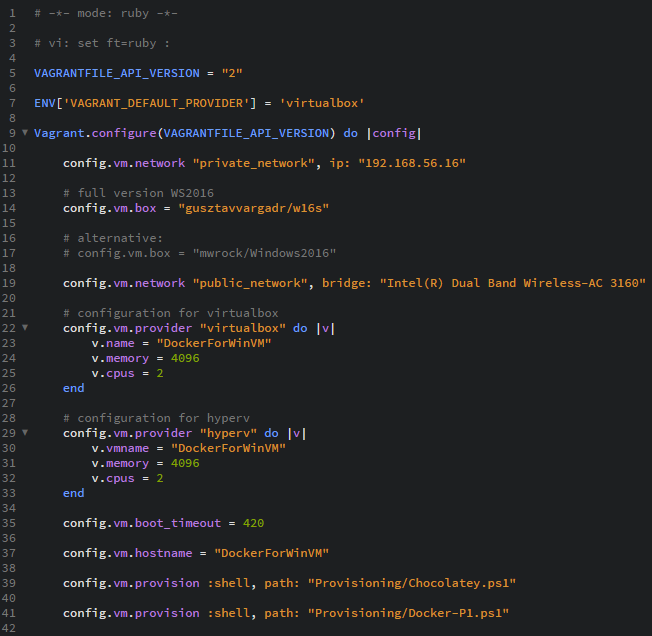
\includegraphics[scale=0.75]{img/windowsvagrant01}
\end{center}

Uitzonderlijk voor de Windows Server wordt er ook gebruik gemaakt van een plug-in voor Vagrant, namelijk, de 'Vagrant Reload'-plug-in van Aidan Nagorcka-Smith. Hiermee kan men het 'Vagrant Reload'-commando uitvoeren tijdens het uitrollen van de Vagrant Image naar een Box. Dit is een belangrijke voorwaarde, want de Windows Server dient heropgestart te worden naar de installatie van Docker.

Daarnaast dient er ook gebruik gemaakt te worden van een klein .BAT-script om docker-compose te installeren via pip.

%% foto + code provision
\begin{center}
	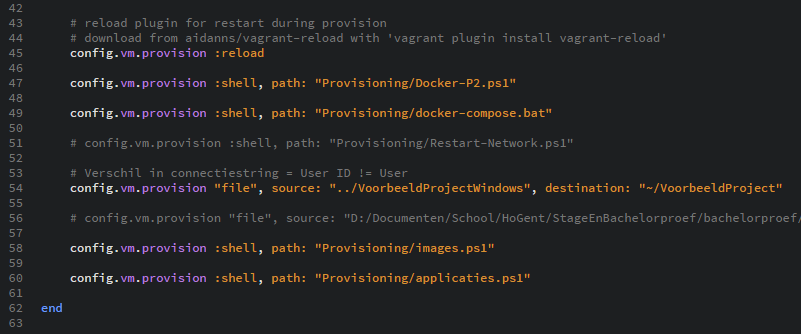
\includegraphics[scale=0.75]{img/windowsvagrant02}
\end{center}

Ten slotte wordt er ook gebruik gemaakt van een reeks provision-commando's om het systeem te voorzien van de nodige scripts en een voorbeeld-project. Het voorbeeld-project bevat een .NET-webapplicatie, die de onderstaande startpagina zou moeten tonen:

%% foto start pagina
\begin{center}
	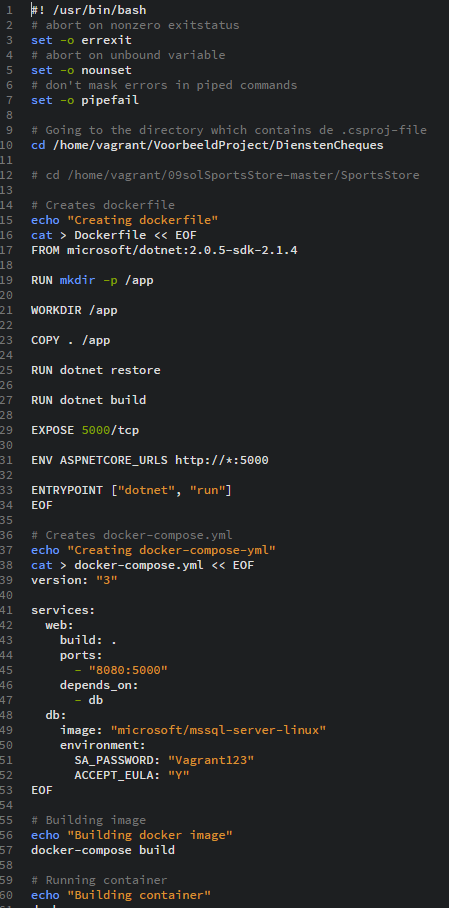
\includegraphics[scale=0.6]{img/centosapplicaties01}
\end{center}

\subsection{PowerShell}
De 6 scripts die voorzien worden, configureren elk een component dat nodig is om de omgeving af te werken.

\begin{itemize}[noitemsep]
	\item Chocolatey
\end{itemize}

In dit script wordt er gekeken of Chocolatey al geïnstalleerd is. Zoja, wordt er gecontroleerd of Chocolatey reeds up to date is, en anders installeert het de packet manager.

\begin{center}
	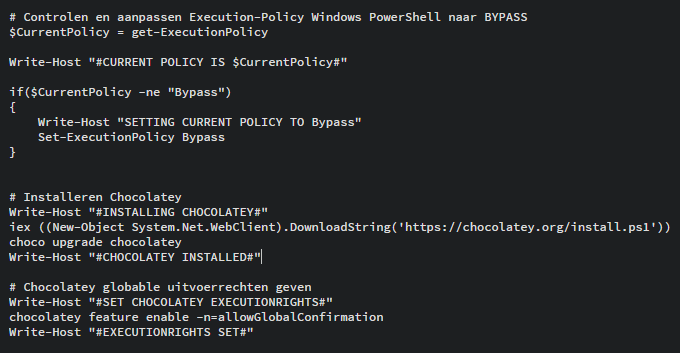
\includegraphics[scale=0.6]{img/chocolatey}
\end{center}

\begin{itemize}[noitemsep]
	\item Docker \#1
\end{itemize}

Hierna wordt het eerste deel van de Docker installatiescripts uitgevoerd. Dit installeert Docker en geeft daarna een melding dat er een reboot aan komt.

Nadat Docker geïnstalleerd is, vereist het systeem namelijk dat het opnieuw wordt opgestart. Deze plug-in is de makkelijkst gevonden manier, zonder in te grijpen in het automatisatie-proces.

\begin{center}
	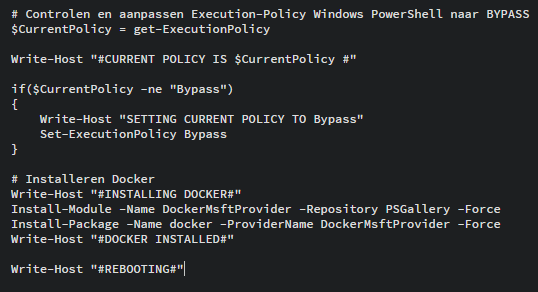
\includegraphics[scale=0.6]{img/docker01}
\end{center}

\begin{itemize}[noitemsep]
	\item Docker \#2
\end{itemize}

Vervolgens wordt Posh-Docker geïnstalleerd. Deze tool voorziet de installatie van Python en Pip door gebruik te maken van Chocolatey. Daarnaast wordt er in dit script ook getest of Docker correct is geïnstalleerd en worden de firewall-rules ingesteld.

\begin{center}
	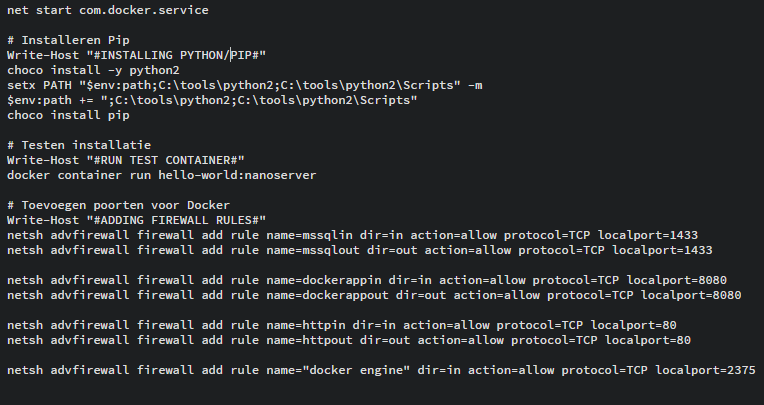
\includegraphics[scale=0.6]{img/docker02}
\end{center}

\begin{itemize}[noitemsep]
	\item docker-compose.bat
\end{itemize}

Hierna wordt het docker-compose.bat-script uitgevoerd. Dit script maakt gebruik van Pip om docker-compose te installeren.

\begin{center}
	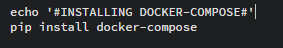
\includegraphics[scale=0.6]{img/dockercompose01}
\end{center}

\begin{itemize}[noitemsep]
	\item Images
\end{itemize}

Vervolgens wordt het Images.ps1-script uitgevoerd. Dit script is verantwoordelijk voor het installeren van de container waarin de databank wordt gehost die de applicatie nodig heeft. Dit gebeurt aan de hand van een Microsoft SQL server Docker Image die van het internet wordt gehaald en waar vervolgens een container mee wordt gebouwd.

\begin{center}
	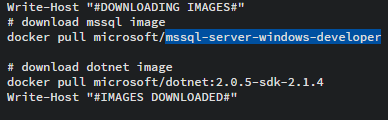
\includegraphics[scale=0.6]{img/dockerimages}
\end{center}

\begin{itemize}[noitemsep]
	\item Application
\end{itemize}

Ten slotte haalt het laatste script die specifieke .NET-sdk Docker Image op die nodig is om de container te bouwen die de webapplicatie vereist. Daarna maakt het script de Dockerfile aan en vult deze op met de vereiste tekst om de container te bouwen, alsook de commando's om daarna de Docker Image en Container te bouwen.

\begin{center}
	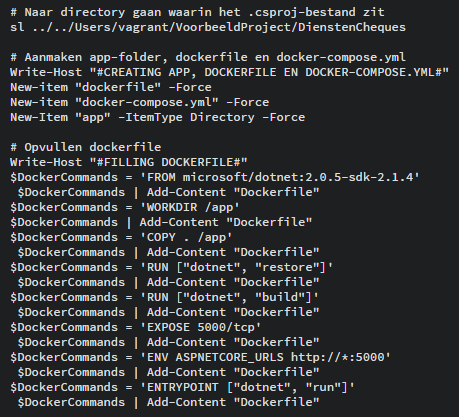
\includegraphics[scale=0.6]{img/dockerfile01}
\end{center}

\begin{center}
	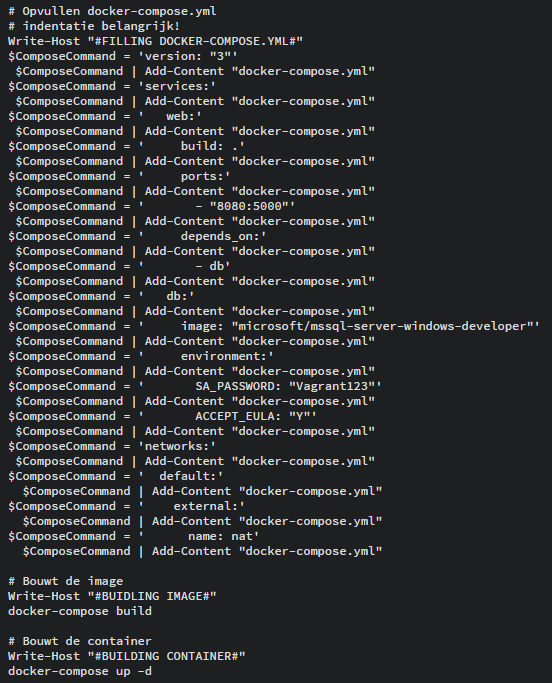
\includegraphics[scale=0.6]{img/dockerfile02}
\end{center}

\section{CentOS 7.4}
%% hardware
%% software
%% vagrant (code + foto)
%% Bash (code + foto)

\subsection{Vagrant}
Om de CentOS-server te installeren wordt er gebruik gemaakt van de officiële Vagrant Image die beschikbaar wordt gesteld door de organisatie achter CentOS, namelijk Red Hat Enterprise Linux (RHEL). Deze voorziet alleen een basis installatie van een CentOS 7.4 server, maar voorziet wel de mogelijkheid om uitgerold te worden op alle populaire platformen.

%% foto + code
\begin{center}
	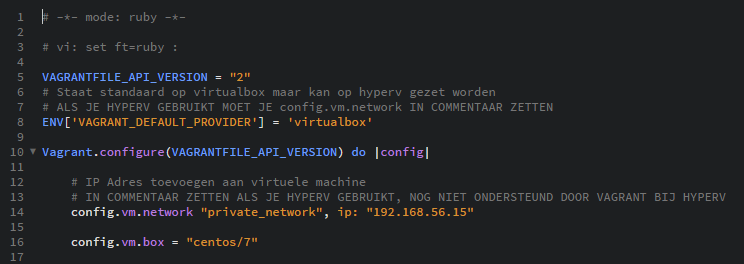
\includegraphics[scale=0.75]{img/centosvagrant01}
\end{center}

Ook hier krijgt het systeem 4GB RAM en 2 cores, zodat er op een eerlijke manier naar de performantie van beide systemen kan worden gekeken. Verder krijgt het systeem ook een hostname en VMName.

%% foto + code
\begin{center}
	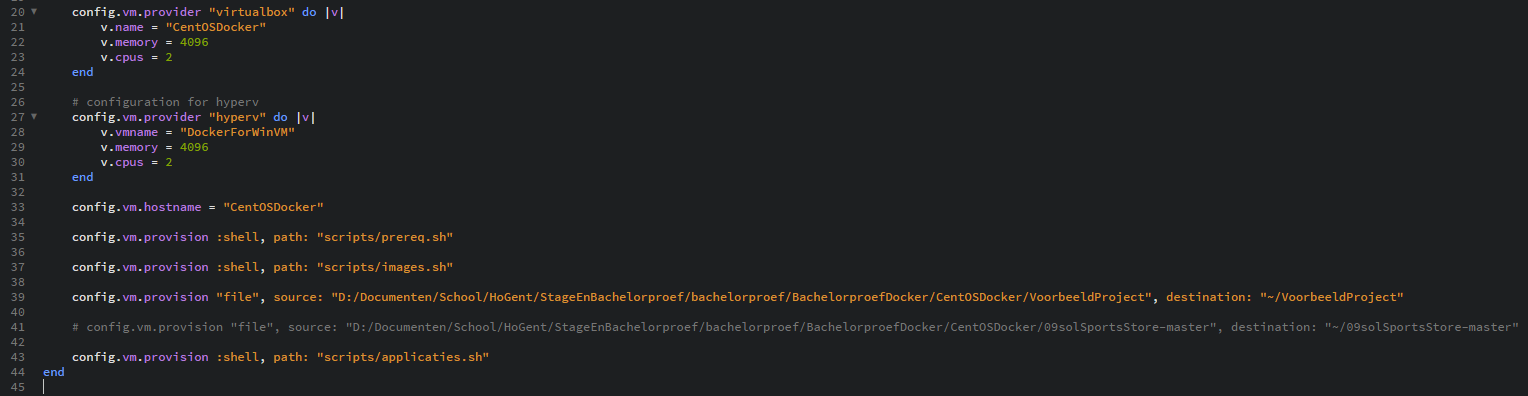
\includegraphics[scale=0.6]{img/centosvagrant02}
\end{center}

Ten slotte worden er 3 scripts voorzien bij het provision-gedeelte, zodat alle benodigde componenten kunnen worden geïnstalleerd. Hieronder behoort onder andere een script om dezelfde webapplicatie te voorzien als voor Windows.

\subsection{Bash}

\begin{itemize}[noitemsep]
	\item prereq
\end{itemize}

In dit gedeelte van het script worden alle functionaliteiten voorzien die nodig zijn voordat men kan beginnen aan het uitrollen van de applicatie, waaronder de installatie van Docker, docker-compose, Epel-Release, Git, Nano en anderen.
Daarnaast worden ook regels toegevoegd aan de firewall, zodat de container beschikbaar is nadat deze volledig is opgesteld.

\begin{center}
	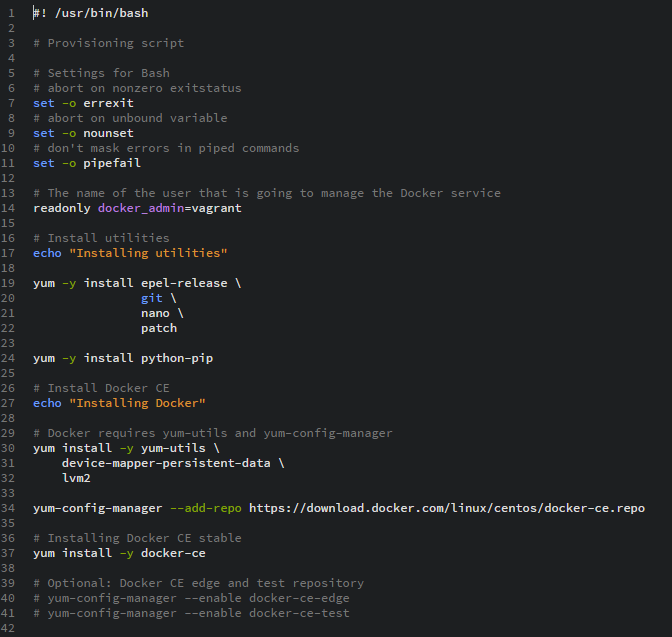
\includegraphics[scale=0.6]{img/centosprereq01}
\end{center}

\begin{center}
	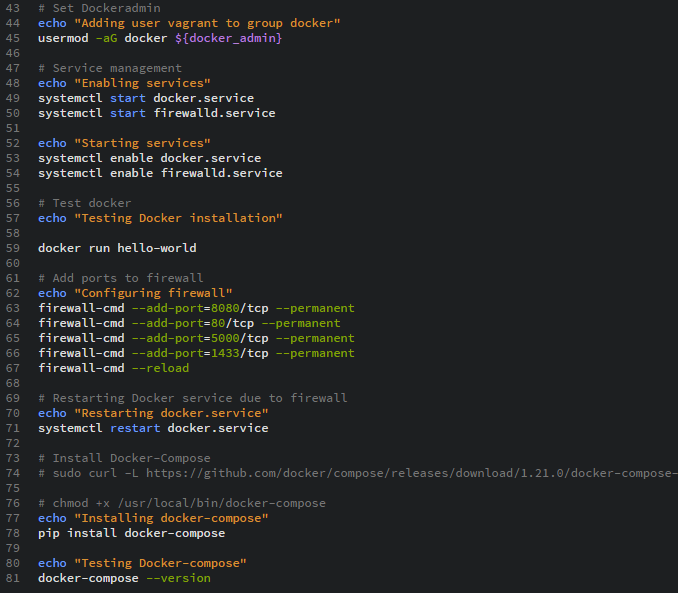
\includegraphics[scale=0.6]{img/centosprereq02}
\end{center}

\begin{itemize}[noitemsep]
	\item images
\end{itemize}

Bij het volgende script worden alle Docker Images van Docker Hub gehaald, wat de officiële online repository van Docker is waar alle beschikbare Docker Images op staan.

\begin{center}
	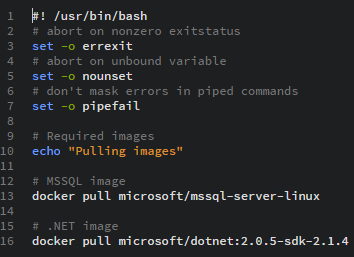
\includegraphics[scale=0.6]{img/centosimages01}
\end{center}

\begin{itemize}[noitemsep]
	\item applicaties
\end{itemize}

Ten slotte worden in het laatste script de benodigde databank en applicatie omhoog gebracht aan de hand van een dockerfile, docker run- en docker build-commando's.
De dockerfile- en dockercompose.yml-bestand worden opgevuld met een 'EOF' identifier. Hierdoor blijft Bash de invoer pipen in de dockerfile tot hij 'EOF' tegenkomt, waarna hij stopt zonder 'EOF' mee te nemen.

\begin{center}
	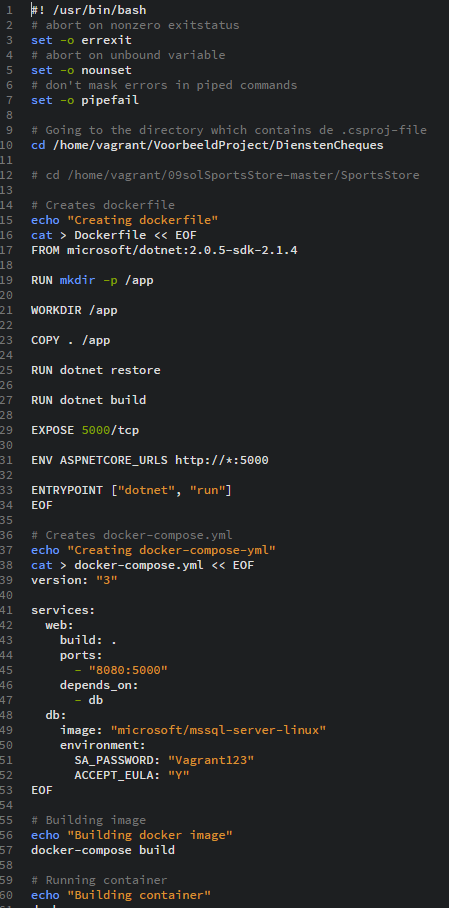
\includegraphics[scale=0.6]{img/centosapplicaties01}
\end{center}